\documentclass[runningheads]{llncs}

\usepackage[T1]{fontenc}
\usepackage{graphicx}
%
\begin{document}
%
\title{Expanding Flicker30k: a Novel Dataset for Persian Language Captions}
%
%\titlerunning{Abbreviated paper title}
% If the paper title is too long for the running head, you can set
% an abbreviated paper title here
%
\author{Shima Baniadamdizaj\inst{1}\orcidID{0000-0003-1678-5108} \and
Alexander Breuer\inst{1} }
%
\authorrunning{Sh. Baniadamdizaj et al.}
% First names are abbreviated in the running head.
% If there are more than two authors, 'et al.' is used.
% 
\institute{Friedrich Schiller University Jena, Jena, Germany \\
\email{\{sima.bani, alex.breuer\}\@uni-jena.de}}
%
\maketitle              % typeset the header of the contribution
%
\begin{abstract}
Image captioning, the challenge of describing images through natural language, particularly benefits from deep learning techniques which needs diverse datasets. While existing datasets like Microsoft COCO and Flickr30k offer valuable resources, they are predominantly in English. The Expanding Flicker30k dataset fills this void for the Persian language. With manually curated captions averaging 13.3 words, the dataset captures various visual scenarios. By addressing the absence of Persian captioning resources, this paper contributes to both image captioning and multi-lingual research, fostering improved image understanding and language generation capabilities.
This paper presents a novel resource for Persian language image captioning. Built upon the Flickr30k dataset, the new collection comprises 51,000 captions corresponding to 10,200 distinct images, providing a crucial dataset for advancing image captioning research in the Persian language. Each picture has five captions in Persian, which helps overcome the lack of non-English captioning datasets and allows for detailed language analysis. The dataset includes columns for image names, comment numbers, Persian captions, and English translations, facilitating bilingual comparisons.

\keywords{Image Captioning in Persian \and Computer Vision \and Natural language processing \and image-to-text.}
\end{abstract}
%
%
%
\section{Introduction}
% \subsection{A Subsection Sample}
Image captioning involves the automated process of describing image content using natural language sentences. While humans effortlessly understand images, machines struggle to generate informative captions. They must grasp semantic relationships between objects, attributes, and actions to create coherent descriptions, a task humans find easy. Additionally, machines must convert these semantic relations into accurate literature. For example, an appropriate caption for an image with a train and people at a station might describe people boarding the train or waiting on the platform.

Image captioning predominantly relies on deep learning techniques \cite{Karpathy2015,Vinyals2015,Xu2015,Luo2023}. Successful deep learning-based captioning necessitates vast image datasets for effective model training. Diverse image sources such as TV, internet, and news lack accompanying descriptions. Captioned image datasets like Microsoft COCO \cite{MSCOCO}, Flickr8k \cite{Flickr8k}, and Flickr30k \cite{Flickr30k} provide valuable resources for training. These datasets, comprising diverse images with human-generated captions, facilitate accurate captioning model development.

Despite abundant English datasets, scarcity prevails in large-scale non-English image captioning datasets.For instance, the Multi30k dataset \cite{Multi30k}, encompassing English-German captions. Translating English datasets into other languages offers a cost-effective approach for non-English captions. Studies \cite{Xue,Zoph,Rosa} indicate that translated datasets can impact model performance negatively. Addressing the scarcity of Persian image captioning datasets, we present a dataset based on Flickr30k \cite{Flickr30k}. This dataset of 10,180 images with Persian captions is the first proposed solution for global image captioning in Persian. Each image has five reference descriptions, averaging 13.3 words with a standard deviation of 5.5 words. Notably, Persian prepositions are distinct words separated by spaces.

This paper comprises five chapters, each vital to exploring Persian image captioning. Chapter 1 introduces the research and stresses the need for a dedicated dataset. Chapter 2 explores motivation, related works, and existing datasets, emphasizing the gap for a Persian dataset. Chapter 3 details dataset collection, annotation, and preprocessing. Chapter 4 presents experiments, discussions, and analyses. Chapter 5 concludes and outlines future prospects. This work contributes a resource for Persian language visual understanding and bridges the gap in image captioning research.

% Chapter 2
\section{Motivation and Related Works}
The machine's ability to perform image captioning has been greatly facilitated by the availability of large-scale annotated datasets. Some well known examples of such datasets in English language are Microsoft COCO \cite{MSCOCO}, Flickr8k \cite{Flickr8k} and Flickr30k \cite{Flickr30k}. Despite the existence of non-English image captioning datasets, such as Multi30k \cite{Multi30k} and VIST \cite{VIST} for English-German and English-Chinese captions, respectively, there is still a noticeable scarcity of Persian language datasets. The availability of large-scale captioning datasets specifically in Persian is limited, which presents a challenge for training models to generate captions in this language.

\subsection{English Captioned Datasets}
MS COCO (Microsoft Common Objects in COntext) \cite{MSCOCO} is a widely used computer vision dataset containing over 164k diverse images. Sourced from various platforms, it offers comprehensive annotations, including precise bounding boxes for object detection and segmentation masks. The dataset's training set comprises approximately 83k images, while both the validation and test sets contain around 41k images each. The average description length is about 10 words. It finds applications in object recognition, scene understanding, and image captioning, contributing significantly to advancements in computer vision research.

Flickr8k \cite{Flickr8k}, another significant computer vision dataset, focuses on image captioning. Curated for this task, it boasts a collection of 8k high-quality images drawn from the popular photo-sharing platform Flickr. Each image is accompanied by five human-generated captions, creating a rich source of textual descriptions for the visual content. This dataset is carefully designed to encompass a wide range of scenes, objects, and activities, showcasing the diverse nature of real-world imagery. It serves as a crucial resource for training and evaluating image captioning models, playing a pivotal role in the development of algorithms that generate contextually relevant and accurate image descriptions. The availability of Flickr8k has played a key role in advancing the realms of image captioning, natural language understanding, and computer vision as a whole.

Alongside the Flickr8k dataset, there exists a more expansive counterpart called Flickr30k \cite{Flickr30k}. While Flickr8k contains 8,000 images, Flickr30k significantly surpasses it with around 30,000 images, offering a substantial augmentation in scale. Both datasets share Flickr as their source and aim to encompass diverse scenes and objects within their contextual milieu, accompanied by human-generated captions.
However, Flickr30k's increased size brings several distinct advantages. Its content diversity bolsters the resilience and applicability of computational models across intricate computer vision tasks. The broader range of images covers an array of real-world scenarios and concepts, empowering researchers to tackle intricate challenges in object recognition, scene comprehension, and image captioning. In essence, Flickr30k's expansion not only enriches the dataset but also stimulates comprehensive research and innovative problem-solving.

"Nocaps" \cite{Nocaps} emerges as a dedicated dataset for the domain of image captioning. It sets its focus on the realm of novel and diverse scenes, aiming to expand the horizons of captioning models in handling an even wider array of images and contexts effectively. The dataset encompasses a vast collection of images, each coupled with multiple human-generated captions. A grand total of 166,100 captions accompany 15,100 images, spanning over 500 unique object classes. These images are sourced from the Open Images V4 \cite{Openimages}, a publicly available dataset tailored for large-scale multi-label and multi-class image classification tasks. Open Images V4 enriches the dataset with a diverse spectrum of visual concepts, guaranteeing a comprehensive representation of real-world objects and scenes. This broader scope is cemented by the dataset's impressive compilation of 1.9 million images, each capturing complex scenes.

Some datasets cater to specific use cases. The VizWiz-Captions dataset \cite{VizWiz}, for instance, is meticulously crafted to address the distinct challenges faced by individuals with visual impairments when engaging with visual content. The dataset boasts an assemblage of approximately 31k images, with each image complemented by a human-generated caption. Notably, the VizWiz and MS COCO datasets exhibit an overlap of about 54\% concerning the provided captions. Images and captions for the VizWiz-Captions dataset stem from the VizWiz mobile application, a platform that empowers visually impaired users to capture images and inquire about content through questions. This unique dataset is indispensable for driving advancements in accessibility and inclusivity within the realm of computer vision and natural language processing.

The mentioned datasets have limitations, as they provide captions for only English speakers. This lack of other language representation shows the necessity of the development of image captioning datasets for non-English speakers. This will enable a more comprehensive and inclusive environment for advancing image captioning task, and provide a wider accessibility and applicability across different languages.

\subsection{Non-English Image Captioning Datasets}
In the context of lacking a Persian image captioning dataset, this section focuses on non-English alternatives, emphasizing the need for Persian-specific datasets.

The Multi30k dataset \cite{Multi30k} stands as a prime example. Renowned for image captioning and multimodal translation, it extends Flickr30k \cite{Flickr30k}, offering English-German captions. This aids in refining captioning models for both languages.

Another case is the Korean Tourist Spot (KTS) \cite{Korean} dataset, rich in images, textual descriptions, hashtags, and likes. It's customized for exploring Korean tourist spots, with 10 classes and 10,000 instances sourced from Instagram.

Moreover, the ImageCLEF 2018 \cite{ImageCLEF2018} dataset is significant. With 232,305 biomedical image-caption pairs from PubMed Central, it's partitioned into training (222,305 pairs) and test (10,000 pairs) sets. Notably, it spans various languages used in biomedical research, enhancing its utility in diverse linguistic contexts.

\subsection{Persian Image Captioning Datasets}
Datasets such as MS COCO and Flickr have multiple unofficial versions available for various languages, but no Persian. The lack of a Persian language image captioning dataset highlights the need for developing datasets specifically designed for Persian in image captioning tasks. Considering both native and second language speakers, it is estimated that there are approximately 110 to 120 million Persian language speakers worldwide. This includes native speakers from Iran, Afghanistan, and Tajikistan, as well as second language speakers through education, migration, interest, or cultural affinity.

The collection of an image captioning dataset in Persian holds importance for several reasons. Developing an image captioning dataset in Persian, one of the widely spoken languages in the Middle East and Central Asia, addresses the need for natural language processing in this language for the Persian-speaking population and development in AI research. A Persian image captioning dataset opens doors for various practical applications, including content recommendation systems, image search engines, accessibility tools for visually impaired individuals, and language learning platforms which currently are not supporting this language.

Moreover, creating a Persian image captioning dataset promotes cultural preservation and representation. Persian culture encompasses a rich heritage of art, traditions, and historical landmarks. By focusing on images relevant to Persian culture and context, we capture the essence of Persian identity and contribute to preserving and showcasing its visual heritage. This dataset is valuable for documenting, educating about, and promoting Persian culture.

In conclusion, the collection of an image captioning dataset in Persian addresses the specific linguistic and cultural needs of the Persian-speaking community. It enables development in AI research, and contributes to the preservation and promotion of Persian cultural heritage. By undertaking this endeavor, we aim to bridge the language gap in how images are understood and make AI technologies more accessible and inclusive for everyone.

\section{Dataset Description}
The following section presents the detailed data collection and analysis procedures. The dataset comprises a collection of images that were exclusively sourced from Flickr30k \cite{Flickr30k}. This section focuses on detailing the process of data collection and labeling, specifically for Persian image captioning. The aim is to provide a comprehensive understanding of the procedure followed to gather the dataset.

To initiate the data collection process, various sources were explored to obtain a diverse range of images suitable for Persian image captioning. Special attention was given to selecting images that represented a broad spectrum of subjects, scenarios, and contexts, ensuring the dataset's comprehensiveness and inclusivity.
% There is one example from dataset in Fig.~\ref{fig1}. 

% \begin{figure}[htbp]
%   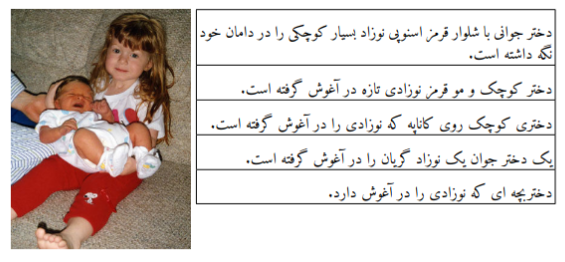
\includegraphics[width=\textwidth]{fig1.png}
%   \caption{Example image from the dataset with relative captions.}
%   \label{fig1}
% \end{figure}

\subsection{Image Collection}
This paper focuses on the collection and annotation of a dataset of images sourced from Flickr30k \cite{Flickr30k} which contains a diverse community of photographers and accordingly photos. Both amateur enthusiasts and seasoned professionals contribute to this platform, resulting in a rich and varied collection of photos. This feature ensures representation across a wide array of visual attributes. These sources were carefully chosen to ensure the availability of high-quality images aligned with the desired scope of the study.

Additionally, these selected images were carefully chosen to contain various situations and were annotated by human annotators same as the original dataset (Flicker30k). By using some of the images from the Flickr dataset, we enable multitask learning and transfer learning approaches for image captioning tasks involving two languages (English/ Persian).

\subsection{Annotation Procedure}
The annotators were instructed to describe the images using words or sentences that accurately depicted the content, focusing on the most important aspects of each image. Annotators fluent in Persian were asked to do a captioning task to ensure the captions accurately reflect the semantic meaning and context of the images, including grammar, syntax, and nuances. Each image in the dataset is annotated with five different captions. Although some captions may have similarities, they are entirely distinct. If duplicate captions were found for an image, one of them was removed, and the annotator was asked to provide a new caption.

To maintain consistency and enhance the overall quality of the dataset, a comprehensive annotation guideline was developed. This guideline provided clear instructions and specifications to the annotators, ensuring uniformity in the captioning process and minimizing variations in style and content. This step was crucial to facilitate the training of machine learning algorithms for automatic image captioning in the Persian language in exact terms. This involved organizing the selected images, collecting relevant metadata, and removing duplicates or any unessential content Through these steps, the dataset was carefully cleaned, standardized, and prepared for further analysis. 

To validate the quality of the captions, we asked evaluators to check some specific criteria. These criteria included checking if the caption accurately described the corresponding image, contained at least one word, is grammatically correct, and does not contain any foreign language or harmful content. 

As a result, by carefully following this data collection and captioning procedure, a robust dataset for Persian image captioning was created which provides a resource for training and evaluating machine learning models in the context of automatic image captioning in the Persian language. This dataset can potentially serve as a bilingual (English/ Persian) dataset for various tasks such as image captioning and image description.

\subsection{Content Analysis}
The captioning dataset encompasses 51,000 captions for 10,200 unique images, featuring five distinct captions per image. The dataset is organized into four columns:

\begin{enumerate}
    \item The \texttt{image\_name} column contains image identifiers from the Flickr30k dataset, maintaining original JPG formats and sizes.
    \item \texttt{comment\_number} indicates the count of captions per image, ranging from 0 to 4. Each image hosts five distinct captions.
    \item Persian comments are stored in the \texttt{comment-fa} column, a pivotal contribution of this study.
    \item The \texttt{comment-en} column houses English captions, sourced from the Flickr30k dataset.
\end{enumerate}

During preprocessing, it's important to highlight that the \texttt{comment-fa} column exclusively contains Persian alphabet characters. Numerals are presented in their spelled-out form, ensuring uniformity. Non-word components such as plural indicators aren't included in the word count, while prepositions like "with," "from," or "and" are considered separate words. Caption lengths vary between two and 77 words, with the lengthiest caption attributed to image number 207344485 (as shown in Fig.~\ref{fig2}), spanning 77 words which is:

\begin{figure}[!htbp]
  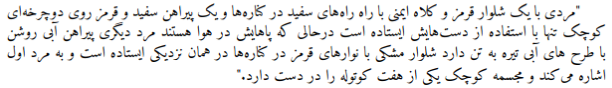
\includegraphics[width=\textwidth]{fig2.png}
\end{figure}

Means: ``A man in red pants and a helmet with white stripes on the sides and a white and red shirt stands on a small bicycle using only his hands while his legs are in the air. Another man wears a light blue shirt with dark blue patterns. Black pants with red stripes on the sides stands nearby, pointing to the first man, holding a small statue of one of the seven dwarfs.''

\begin{figure}
  \begin{center}
    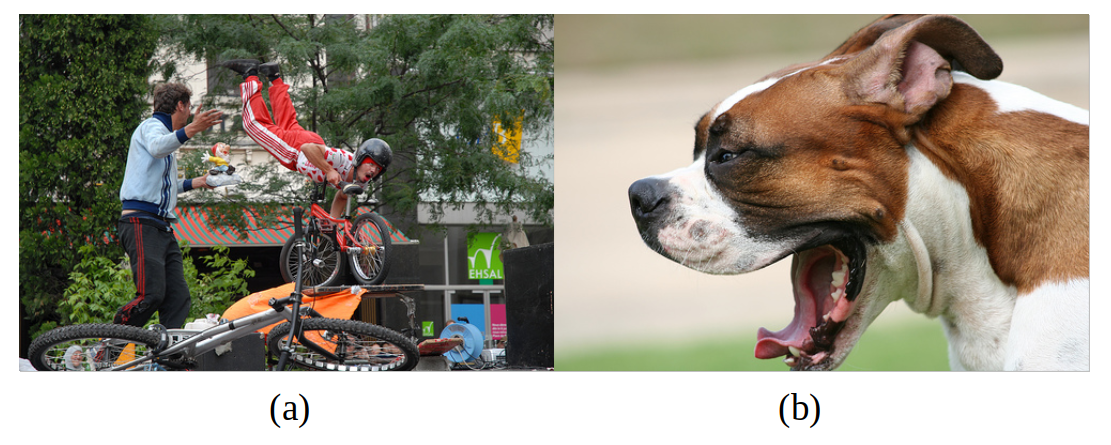
\includegraphics[width=0.8\textwidth]{long_short.jpg}
    \caption{The example images from dataset with (a)longest and (b)shortest Persian captions.} \label{fig2}
  \end{center}
\end{figure}

The shortest captions just contain two words and there are 15 captions with this length which are in the following row numbers: 5801, 6226, 6466, 12606, 13956, 18942, 19937, 25746, 32061, 34616, 38627, 41049, 42221, 44634, and 47940. One of the examples with the shortest caption length is row 34616 in csv file (see Fig.~\ref{fig2}.b): ``Dog's yawn''.

In the proposed dataset, the average word counts per caption is calculated to be 12.33 words. Additionally, the standard deviation of captions lengths is determined to be 5.19. The standard deviation quantifies the extent of variability or dispersion among the caption lengths based ont eh number of words in the dataset. It provides a measure of how spread out the word lengths are from the average value, 12.33, offering insights into the distribution of word lengths and the overall diversity within the dataset (see Fig.~\ref{fig3}).

The dataset analysis shows a diverse range of word lengths in the captions, spanning from two to 77 words per caption. While no specific pattern emerged, varying frequencies of word lengths have been observed. The most frequently occurring word length was nine words, repeating a substantial number of 4808 times. Additionally, lengths 11 and 10 were also prevalent, each repeating 4730 times. Moreover, length eight was observed with a frequency of 4465 repetitions, while length 12 appeared 4201 times. These findings provide a comprehensive overview of the word length distribution within the dataset, showcasing both the range of word counts and the notable occurrences of specific lengths.

\begin{figure}
  \begin{center}
    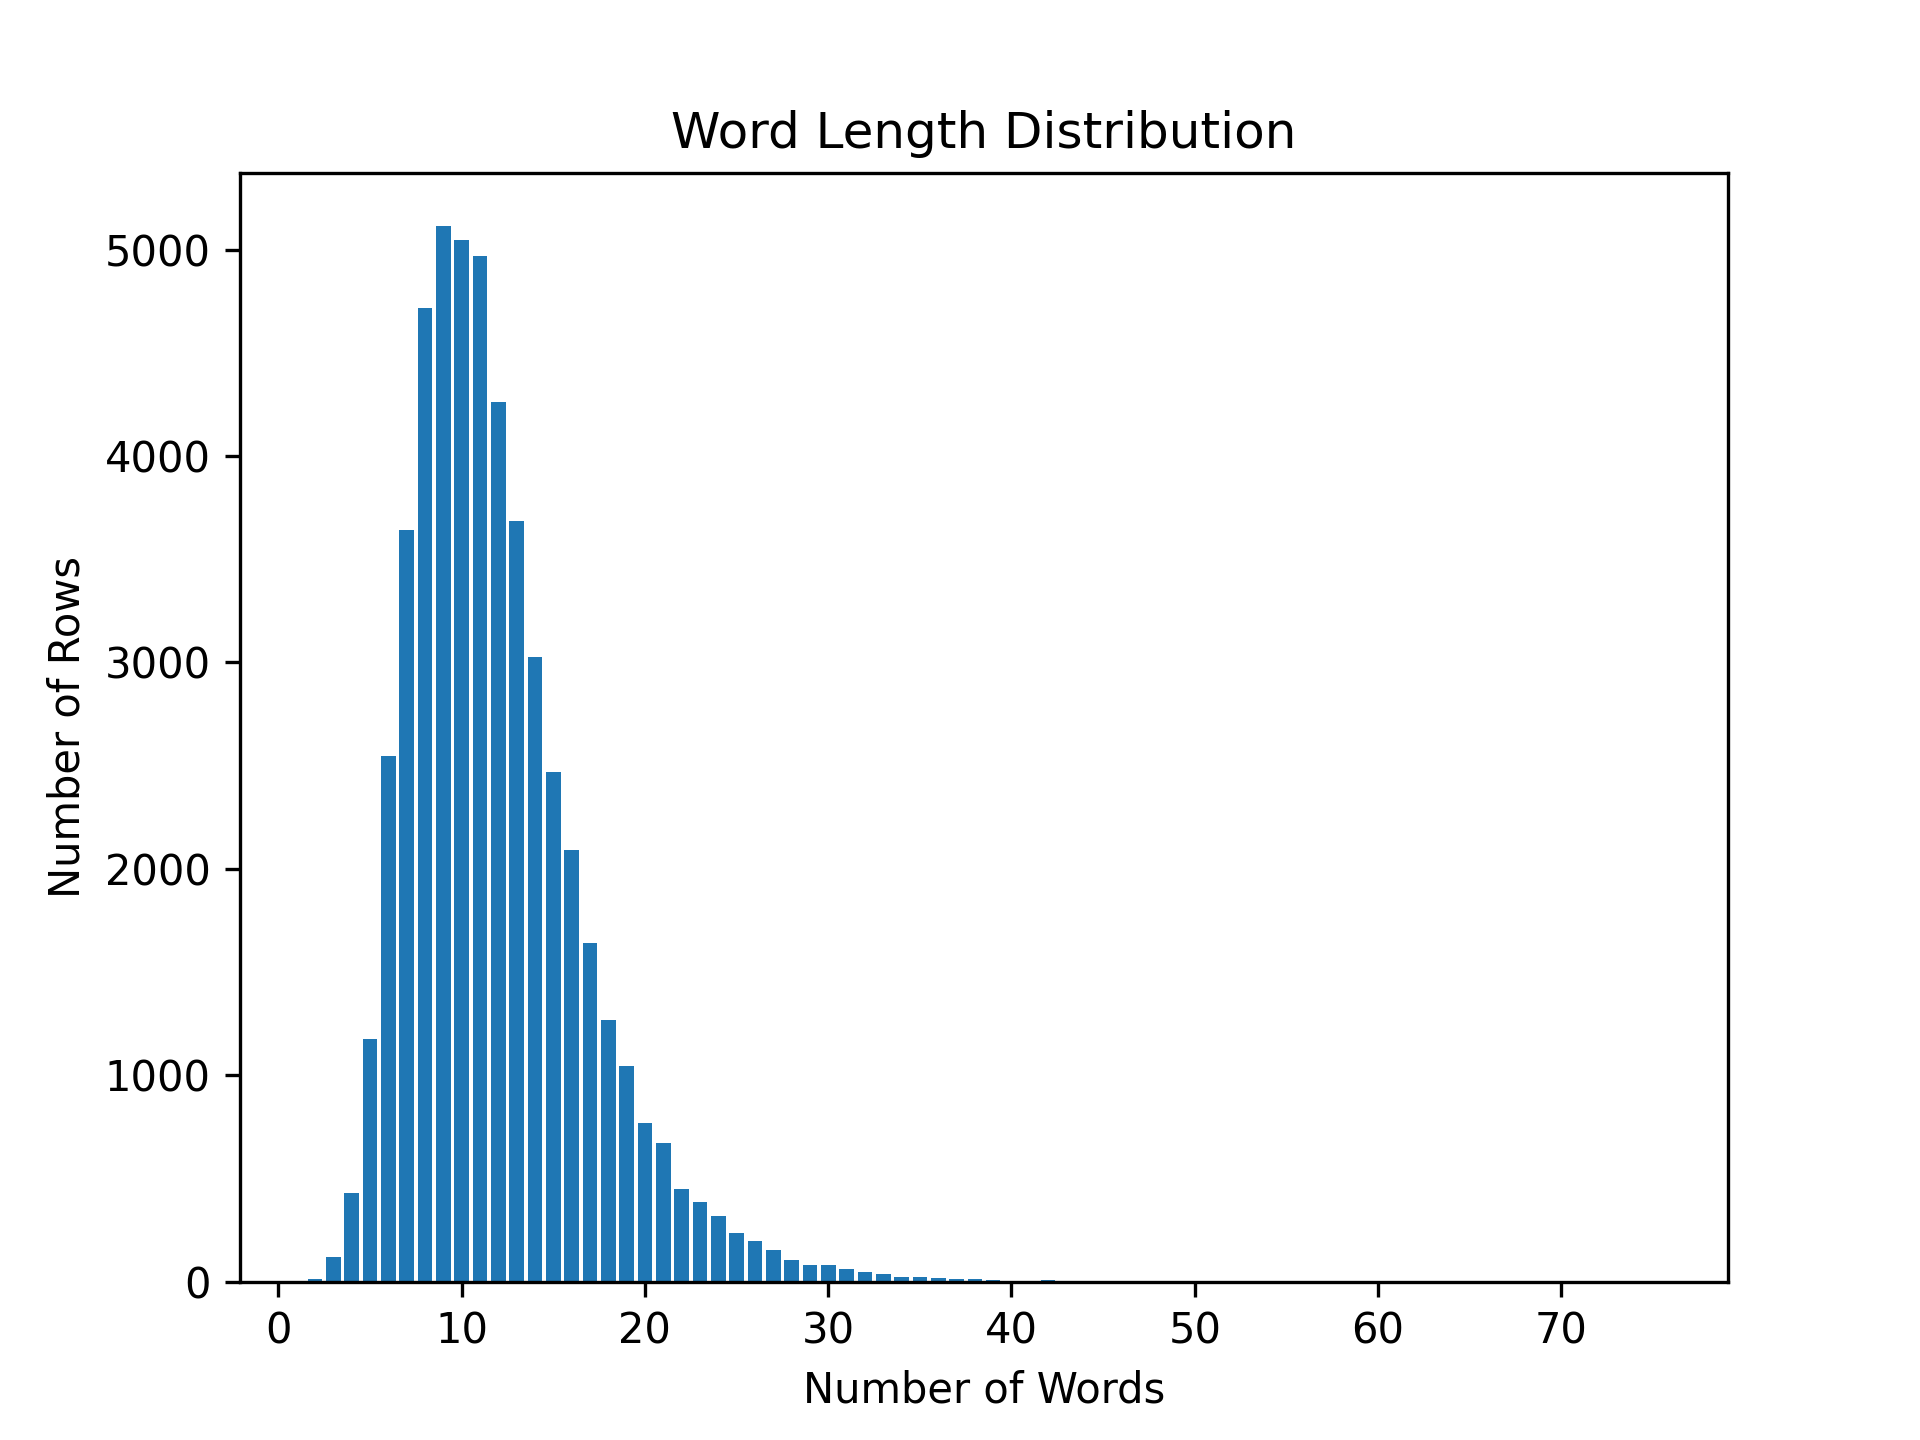
\includegraphics[width=0.6\textwidth]{length_distribution.png}
    \caption{Distribution of word lengths in captions and number of captions per word length.}
    \label{fig3}
  \end{center}
\end{figure}
\vspace{-10pt}

In the dataset analysis, it was observed that certain words appeared with high frequency, indicating their significance in the dataset. The 10 most repeated words are as following: word (a/an) appeared the most, occurring 30,100 times, suggesting its prevalence and potential importance within the context. Similarly, the word (in) was also highly recurrent, appearing 28,029 times. The words (with) and (and) followed closely behind with 21,102 and 20,115 occurrences, respectively, indicating their frequent usage.

Furthermore, the word (that) appeared 19,285 times, highlighting its significance in connecting clauses or introducing relative pronouns. The word (is) occurred 15,473 times, implying its role in expressing existence or attribution. The prepositions (from) and (a particle for direct object) and (to) were also among the most repeated words, with 13,109, 9,974, and 9,615 occurrences, respectively, indicating their frequent usage to denote origin, direct object, and destination.

Additionally, the word (on) appeared 8,996 times, suggesting its relevance in referring to surfaces or indicating location. These findings shed light on the prominent words in the dataset, providing valuable insights into the language patterns and themes present within the text.

\section{Experiments, Results, and Discussions}

This section presents the detailed experiment conducted to develop and evaluate the Persian Image Captioning dataset and its performance using the MobileNetV3Small image feature extractor. It starts by describing the dataset loading process, preprocessing of captions, and the dataset for training and testing. Next, it elaborates on the image feature extraction technique using the pre-trained MobileNetV3Small model. The extracted image features serve as inputs to the subsequent Persian Image Captioning model.

\subsection{Dataset Preprocessing}
The dataset loading utilizes the Python pathlib module, effectively handling file paths. The function extracts content from captions, containing both image filenames and their corresponding Persian captions (five per image). These extracted pairs are organized as tuples, establishing a seamless connection between images and their captions. This alignment ensures precise one-to-one correspondence, enabling streamlined and effective training.

To simplify the retrieval of captions based on image filenames, a specialized Python dictionary is employed. It systematically iterates through the image-caption tuples, appending each caption to the list associated with the relevant image filename key within the dictionary.

Transitioning to text processing, the pivotal tokenization and vectorization process takes center stage. This transformative procedure converts raw text captions into numerical sequences, aligning them for further processing within the Persian Image Captioning model. This task is executed using the TextVectorization layer. Additionally, a layer of standardization is applied to every text caption. This encompasses conversion to lowercase, punctuation removal, and incorporation of \texttt{[START]} and \texttt{[END]} tokens to distinctly mark the inception and conclusion of each caption.

An integral aspect of this preprocessing journey involves vocabulary creation. A vocabulary encompassing the top 10,000 words is established via the TextVectorization layer. This vocabulary constitutes a comprehensive representation of the unique words embedded within the captions, providing a pivotal foundation for subsequent processing stages.

\subsection{Image Feature Extractor}

After loading the dataset, images are processed through the MobileNetV3Small model, a pre-trained model for image classification. The classification layer is turned off, using the last layer's feature-maps as image features. Images are resized to (224x224x3), then batched to (1x224x224x3) for efficient training. Each image becomes a tensor of shape (1x7x7x576), with a grid of 576 feature maps. These features train the Persian Image Captioning model.

\subsection{Transformer-decoder architecture}

The model employs a two-layer Transformer-decoder structure to create captions for input images, comprising key components: Input, Decoder, and Output. The Input involves token embedding and positional encoding. It embeds token IDs and positional data for input text sequences, blending two embeddings. First, Token Embedding retrieves the embedding vector for each token ID using Keras' Embedding layer with \texttt{mask\_zero=True}. Second, Positional Embedding retrieves an embedding vector for each sequence position using the Embedding layer with \texttt{max\_length} as input dimension and \texttt{depth} as output dimension. Position embeddings are learned during training, aiding the model in generalizing to longer sequences.

The decoder has DecoderLayers, each with three sublayers: Causal Self-Attention, Cross Attention (to input image), and FeedForward. This allows the model to use image features and generated text while producing captions.

The model does multiclass classification over the output vocabulary to create captions for input images. The output layer's design is not fully provided here but usually includes a Dense layer followed by softmax activation to compute the word probability distribution in the vocabulary.

\subsection{Model Specifications}

The model employs a two-layer Transformer-decoder structure and incorporates a temperature parameter that facilitates blending among three decoding methods: Greedy Decoding (temperature = 0.0), Random Sampling (temperature = 1.0), and Uniform Random Sampling (temperature > 1.0).

Before commencing training, the model necessitates compilation with specific settings. The chosen optimizer is the \texttt{Adam Optimizer}, an extended version of stochastic gradient descent (SGD), amalgamating adaptive learning rates and momentum. A learning rate of $1 \times 10^{-4}$ is employed. The optimization process employs the softmax cross-entropy loss to gauge dissimilarity between true labels and model-predicted logits. Common in multi-class classification tasks, this function accommodates integer-based ground truth labels.

Following initial loss calculation, a mask is generated to sift out select tokens within the input sequence. The mask hinges on two criteria: labels not equal to 0 and loss less than $1 \mathrm{e} 8$. Ensuring attention to the condition loss < $1 \mathrm{e} 8$ during loss calculation is pivotal; it discards implausibly high losses tied to proscribed tokens. This curation thwarts inconceivable losses, bolstering reliability in loss and accuracy computation. This mask primarily excludes tokens with a label of 0 (padding tokens) and manages numerical predicaments tied to excessive losses. Furthermore, model assessment in training employs a customized accuracy metric.

Training data is fed into the model, iterated indefinitely using \texttt{repeat()} to satisfy epoch requirements. Within each epoch, 100 batches are processed, denoted by the \texttt{steps\_per\_epoch} parameter. Validation data similarly undergoes repeated processing, with the \texttt{validation\_steps} parameter set at 20 per epoch. Training encompasses a total of 100 epochs.

To offer real-time insight during training, a Callback mechanism is implemented. Post each epoch, this Callback generates captions for the surfer image, affording assessment of caption quality across multiple iterations. Insights from this Callback facilitate model refinement and progress evaluation, refining caption generation performance.

\subsection{Results}

Following the completion of model training, the progression of loss Fig.~\ref{fig4}.b and accuracy  Fig.~\ref{fig4}.a throughout the training phase. The blue line corresponds to the training results, while the orange line represents the validation results.
As evident from Fig.~\ref{fig4}, the accuracy attained reaches a maximum of approximately 38\%. It is important to note that this work primarily serves as a representation of the dataset, without further optimization efforts to achieve higher accuracy. Nevertheless, the accuracy results are noteworthy considering the limited enhancements made to the model.

\begin{figure}
  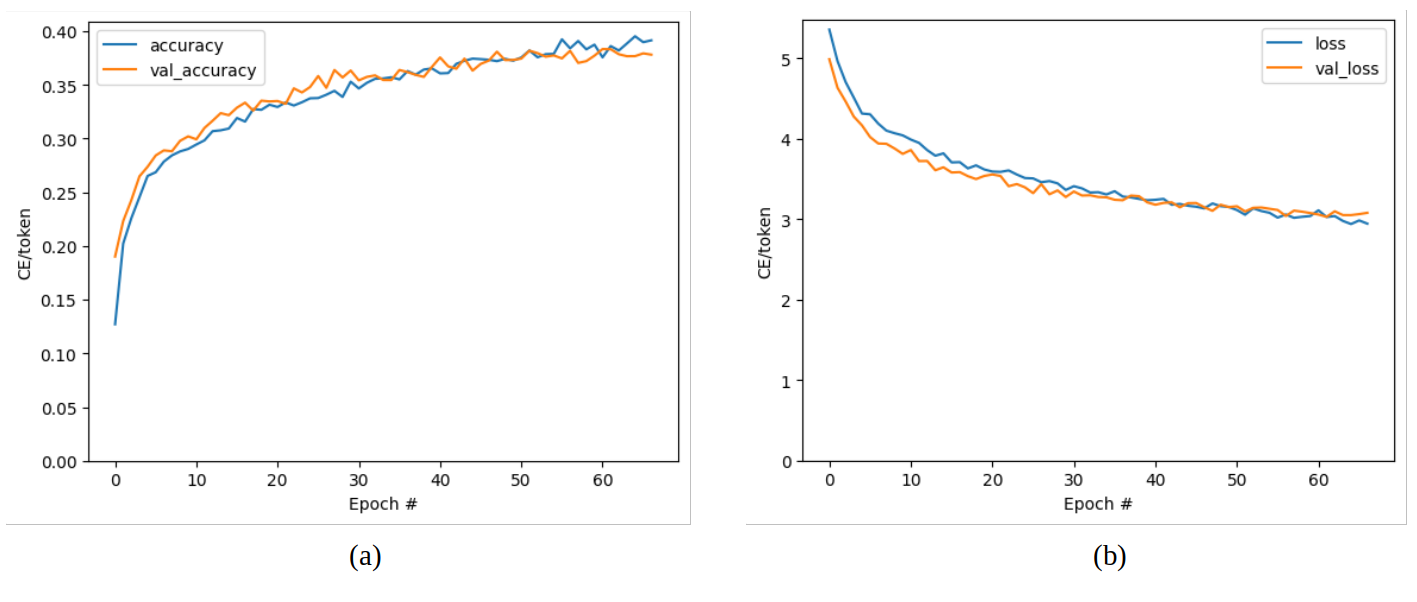
\includegraphics[width=\textwidth]{loss.png}
  \caption{Training and Validation Performance of the Model. The plot displays the changes in accuracy (a) and loss(b) during the training (blue) and validation (orange) process.} \label{fig4}
\end{figure}

Surprisingly, the model's performance on unseen images remains satisfactory. The dataset's focus on dogs, streets, and humans shapes caption generation. The model adeptly produces relevant captions within these constraints. In Fig.~\ref{fig5}, an image portrays an elephant on wetlands mislabeled as a running black dog. Despite misclassification, the caption maintains impeccable grammar. The figure, featuring attention maps, offers insight into the captioning process, even when the model misinterprets the image. This highlights the model's linguistic competence, despite perceptual challenges, enriching understanding of its inner workings.

\begin{figure}
  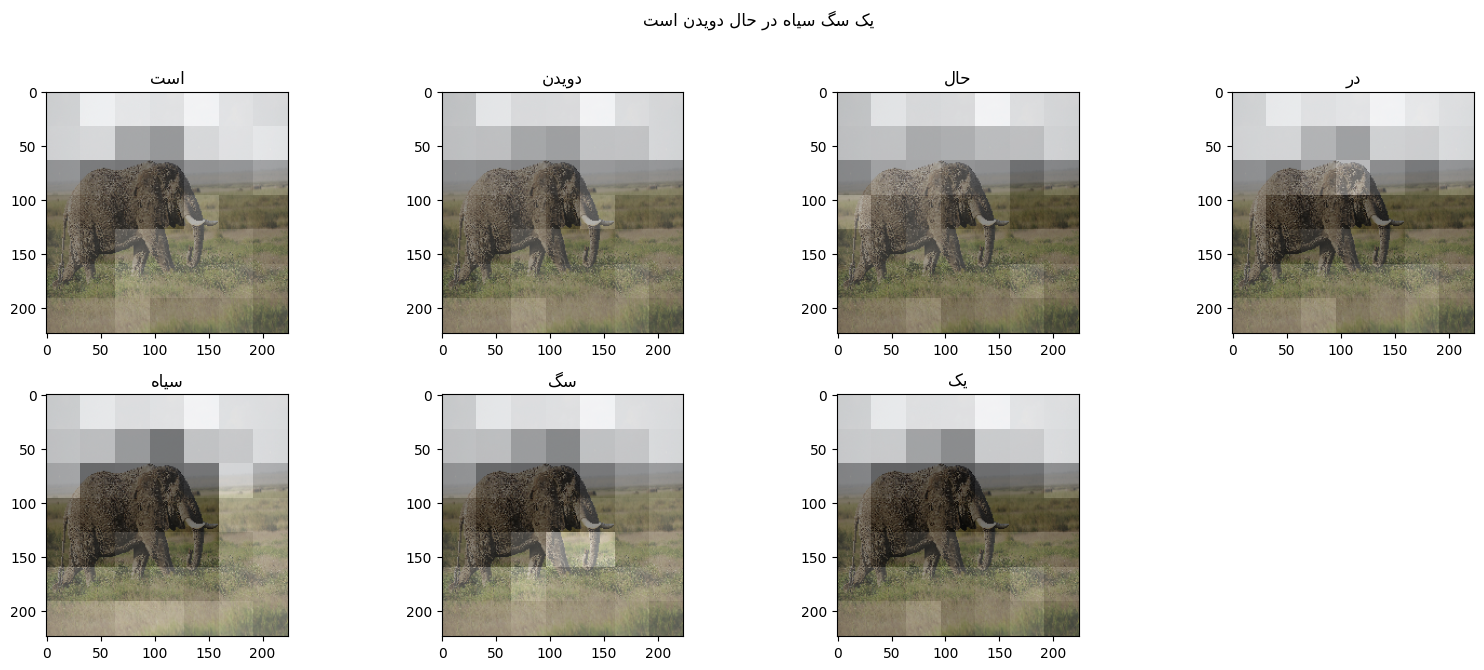
\includegraphics[width=\textwidth]{elephant.png}
  \caption{ Predicted caption and attention maps for captioning an image with an elephant walking.} \label{fig5}
\end{figure}

Furthermore, several additional examples in the dataset highlight the overall accuracy of the provided captions. However, a notable challenge arises from biased images containing specific scenes, leading to misinterpretations by the model. For instance, the model's inability to discern a train from a man or a camera from a machine illustrates the impact of scene biases on the model's comprehension. Addressing these biases becomes imperative to enhance the model's capacity for accurate image captioning in diverse real-world scenarios.

\section{Conclusion and Future Work}
In this paper, a novel dataset for image captioning presented with a specific focus on Persian annotations and sourced from Flicker30k.
In conclusion, the model employed for feature extraction is MobileNetV3Small, coupled with a two-layer transformer decoder network. Despite achieving a modest 38\% accuracy, the model consistently produces grammatically correct captions. Nevertheless, the dataset's limited real-world image representation introduces biases, hindering the model's ability to comprehend certain scenes accurately. To enhance performance, augmenting the dataset with diverse real-world images and exploring more advanced models hold promise for improving accuracy and contextual relevance in image captioning tasks.
Moving forward, our future plans involve expanding the dataset by including a larger number of images and adding multiple captions per image. This expansion aims to enhance the dataset's diversity and provide researchers with a broader range of data to explore. Additionally, we intend to categorize the images into distinct classes, such as landscapes, humans, and animals, for targeted analysis.


% ---- Bibliography ----
\begin{thebibliography}{8}
\bibitem{Karpathy2015}
Karpathy, Andrej, and Li Fei-Fei. "Deep visual-semantic alignments for generating image descriptions." Proceedings of the IEEE conference on computer vision and pattern recognition. 2015.

\bibitem{Vinyals2015}
Vinyals, Oriol, et al. "Show and tell: A neural image caption generator." Proceedings of the IEEE conference on computer vision and pattern recognition. 2015.

\bibitem{Xu2015}
Xu, Kelvin, et al. "Show, attend and tell: Neural image caption generation with visual attention." International conference on machine learning. PMLR, 2015.

\bibitem{Luo2023}
Luo, Jianjie, et al. "Semantic-conditional diffusion networks for image captioning." Proceedings of the IEEE/CVF Conference on Computer Vision and Pattern Recognition. 2023.

\bibitem{MSCOCO}
Lin, Tsung-Yi, et al. "Microsoft coco: Common objects in context." Computer Vision–ECCV 2014: 13th European Conference, Zurich, Switzerland, September 6-12, 2014, Proceedings, Part V 13. Springer International Publishing, 2014.

\bibitem{Flickr8k}
Rashtchian, Cyrus, et al. "Collecting image annotations using amazon’s mechanical turk." Proceedings of the NAACL HLT 2010 workshop on creating speech and language data with Amazon’s Mechanical Turk. 2010.

\bibitem{Flickr30k}
Young, Peter, et al. "From image descriptions to visual denotations: New similarity metrics for semantic inference over event descriptions." Transactions of the Association for Computational Linguistics 2 (2014): 67-78.

\bibitem{Multi30k}
Elliott, Desmond, et al. "Multi30k: Multilingual english-german image descriptions." arXiv preprint arXiv:1605.00459 (2016).

\bibitem{Xue}
Xue, Linting, et al. "mT5: A massively multilingual pre-trained text-to-text transformer." arXiv preprint arXiv:2010.11934 (2020).

\bibitem{Zoph}
Zoph, Barret, and Kevin Knight. "Multi-source neural translation." arXiv preprint arXiv:1601.00710 (2016).

\bibitem{Rosa}
Rosa, Guilherme Moraes, et al. "A cost-benefit analysis of cross-lingual transfer methods." arXiv preprint arXiv:2105.06813 (2021).

\bibitem{VIST}
Huang, Ting-Hao, et al. "Visual storytelling." Proceedings of the 2016 conference of the North American chapter of the association for computational linguistics: Human language technologies. 2016.

\bibitem{Nocaps}
Agrawal, Harsh, et al. "Nocaps: Novel object captioning at scale." Proceedings of the IEEE/CVF international conference on computer vision. 2019.

\bibitem{Openimages}
Krasin, Ivan, et al. "Openimages: A public dataset for large-scale multi-label and multi-class image classification." Dataset available from https://github. com/openimages 2.3 (2017): 18.

\bibitem{VizWiz}
Gurari, Danna, et al. "Captioning images taken by people who are blind." Computer Vision–ECCV 2020: 16th European Conference, Glasgow, UK, August 23–28, 2020, Proceedings, Part XVII 16. Springer International Publishing, 2020.

\bibitem{Korean}
Jeong, Changhoon, et al. "Korean tourist spot multi-modal dataset for deep learning applications." Data 4.4 (2019): 139.

\bibitem{ImageCLEF2018}
Ionescu, Bogdan, et al. "Overview of ImageCLEF 2018: Challenges, datasets and evaluation." Experimental IR Meets Multilinguality, Multimodality, and Interaction: 9th International Conference of the CLEF Association, CLEF 2018, Avignon, France, September 10-14, 2018, Proceedings 9. Springer International Publishing, 2018.

\end{thebibliography}
\end{document}
